
\documentclass[12pt, a4paper]{article}


%%%% Encodings

\usepackage[utf8]{inputenc} % encoding
\usepackage[english]{babel} % use special characters and also translates some elements within the document.

%%%% Misc

\usepackage{hyperref}       % Hyperlinks \url{url} or \href{url}{name}
\usepackage{parskip}        % \par starts on left (not idented)
\usepackage{tocbibind}      % Adds the bibliography to the table of contents (automatically)

% \usepackage[document]{ragged2e}  % Left-aligned (whole document)
% \begin{...} ... \end{...}   flushleft, flushright, center

%%%% Abstract

\usepackage{abstract}       % Abstract

% http://www.ctex.org/documents/packages/special/abstract.pdf
\renewcommand{\absnamepos}{flushleft} % \begin{abstract} \noindent ... \end{abstract}
\setlength{\absleftindent}{0pt}
\setlength{\absrightindent}{0pt}

%%%% Graphics

\usepackage{graphicx}
\graphicspath{ {./images/} } % directory to look up for graphics

% \begin{figure}[h]
%   \centering
%   
\includegraphics[scale=0.5]{cat}  % [width=\textwidth, height=4cm],
%   \caption{Example of a cat}
%   \label{fig:cat}
% \end{figure}

%%%% Math

\usepackage{amsmath}        % Math
\usepackage{amssymb}        % New symbols http://milde.users.sourceforge.net/LUCR/Math/mathpackages/amssymb-symbols.pdf
\usepackage{bm}             % $\bm{D + C}$

\usepackage{amsthm} % Math, \newtheorem, \proof, etc
% \begin{theorem}\label{t:label}  ...  \end{theorem}
% \begin{proof} ... \end{proof}
\theoremstyle{plain} % default
\newtheorem{theorem}{Theorem}[section]
\newtheorem{corollary}{Corollary}[theorem]  % Numering depends on the current section (instead of global)
\newtheorem{lemma}[theorem]{Lemma} % Shares numeration with theorem.
\theoremstyle{definition}
\newtheorem{definition}{Definition}[section]
\theoremstyle{remark}
\newtheorem*{remark}{Remark}

% Defines a new environment to write your or claim - proof
\newenvironment{claim}[1]{\par\noindent\underline{Claim:}\space#1}{}
\newenvironment{claimproof}[1]{\par\noindent\underline{Proof:}\space#1}{\hfill $\blacksquare$}

%%%% Code/Pseudo-code

\usepackage{minted} % Code listing
% \mint{html}|<h2>Something <b>here</b></h2>|
% \inputminted{octave}{BitXorMatrix.m}

%\begin{listing}[H]
  %\begin{minted}[xleftmargin=20pt,linenos,bgcolor=codegray]{haskell}
  %\end{minted}
  %\caption{Example of a listing.}
  %\label{lst:example} % You can reference it by \ref{lst:example}
%\end{listing}

\newcommand{\code}[1]{\texttt{#1}} % Define \code{foo.hs} environment

\usepackage[ruled,vlined]{algorithm2e} % pseudo-code http://tug.ctan.org/macros/latex/contrib/algorithm2e/doc/algorithm2e.pdf

%%%% Colors

\usepackage{xcolor}         % Colours \definecolor, \color{codegray}
\definecolor{codegray}{rgb}{0.9, 0.9, 0.9}
% \color{codegray} ... ...
% \textcolor{red}{easily}

%%%% Math

%\makeglossaries % before entries

%\newglossaryentry{latex}{
    %name=latex,
    %description={Is a mark up language specially suited
    %for scientific documents}
%}

% Referene to a glossary \gls{latex}
% Print glossaries \printglossaries

\usepackage[acronym]{glossaries} %

% \acrshort{name}
% \acrfull{name}
% \newacronym{foo}{arcshort}{acrfull}

\usepackage{enumitem} % \begin{enumerate}[label=(\alph*)]



\usepackage{fancyhdr}
\pagestyle{fancy}
\fancyhf{}
\rhead{Arnau Abella}
\lhead{Randomized Algorithms - UPC}
\rfoot{Page \thepage}

\title{%
  \vspace{-10ex}
  RA: An Exploratory Assignment on Minimum Spanning Trees
}
\author{%
  Arnau Abella \\
  \large{Universitat Polit\`ecnica de Catalunya}
}
\date{\today}

\begin{document}
\maketitle

%%%%%%%%%%%%%%%%%%%%

\vspace{5ex}

%* If you chose to throw away edges, how did you determine `k(n)`, and how effective was this approach?
%* Can you give a rought explanation for your results? (The limiting behaviour as `n` grows large can be proven rigorously, but it is very difficult; you need not attempt to prove any exact result.)
%* Did you have any interesting experiences with the random number generator? Do you trust it?

\section{Introduction}\label{sec:1}

Let the weight of a tree be the sum of the squares of its edges lengths. Given a set of points $P$ in the unit square $I \times I$ let $W(P)$ be the weight of the \textit{minimum spanning tree (MST)} of $P$, where an edge length is the \textit{Euclidean distance} between its endpoints. If $P$ consist of the four corners of the square, then $W(P) = 3$. Gilbert and Pollack \cite{gil68} proved that $W(P)$ is $\mathcal{O}(1)$ and this was extended to an arbitrary number of dimensions by Bern and Eppstein \cite{bern93}. While more recent \textit{divide-and-conquer} approaches have show that $W(P) \leq 4$, no point set is known with $W(P) > 3$, and hence it has been widely conjectured that $W(P) \leq 3$. In 2013, it was proven that $W(P) < 3.41$ \cite{aichholzer2013sum}. Here we show an empirical experiment to check whether $W(P) < 3.41$ holds for any $MST(P)$.

\section{Experiment}\label{sec:2}

In order to check the previous theorem, we uniformaly at random generate points in the unite square $P$ and compute the weight of the $MST$. We do this with an increasing number of points in order to explore the solution space. It is important to note that the exploration is not exhaustive since exploring the whole solution space would require a large amount of computational power. Also, the implementation is na\"ive since it does not explicitly aims for the degenerate instances where $W(P) \sim 3.41$ may happen.

% How the graph is generated

%* What minimmum spanning tree algorithm did you use, and why?
%* What is the running time of your algorithm?

The it uses \textit{Prim's Algorihm} to search for the $MST$ on the unit square.

\begin{algorithm}[H]
  \SetAlgoLined
  \DontPrintSemicolon
  \SetKwInput{Input}{Input}
  \SetKwInput{Output}{Output}
  \Input{An undirected weighted graph $G = (V,E)$}
  \Output{The minimum spanning tree of the input graph $G$}
  \ForEach{$v \in V$}{
    $key(v) = \infty$\;
    $parent(v) = NIL$\;
  }
  $key(r) = 0$ \tcp*[r]{Pick \textit{u.a.r.} the initial vertex $r \in V$}
  $Q = V$\;
  \While{$Q \neq \emptyset$}{
    $u = EXTRACT-MIN(Q)$\;
    \ForEach{$v \in ADJ(u)$}{
      \If{$v \in Q$ and $w(u,v) < key(v)$}{
        $key(v) = w(u,v)$\;
        $parent(v) = u$\;
      }
    }
  }
  \caption{Minimum Spanning Tree Prim's Algorithm}
\end{algorithm}

\begin{table}[H]
  \center
  \begin{tabular}{ccccc}
    $|V|$  & Time       & $R^2$   & $\mu$      & $\sigma$    \\ \hline
    $128$  & $8.1$   ms & $0.996$ & $8.358$ ms & $327.8$ $\mu$ \\
    $512 $ & $406.0$ ms & $1.0  $ & $391.9$ ms & $10.33$ ms    \\
    $1024$ & $153.6$ ms & $1.0  $ & $150.3$ ms & $3.178$ ms    \\
    $2048$ & $943.1$ ms & $1.0  $ & $934.4$ ms & $14.24$ ms
  \end{tabular}
\caption{Prim's Algorithm benchmark.}
\label{table:1}
\end{table}

\begin{figure}[H]
  \center
  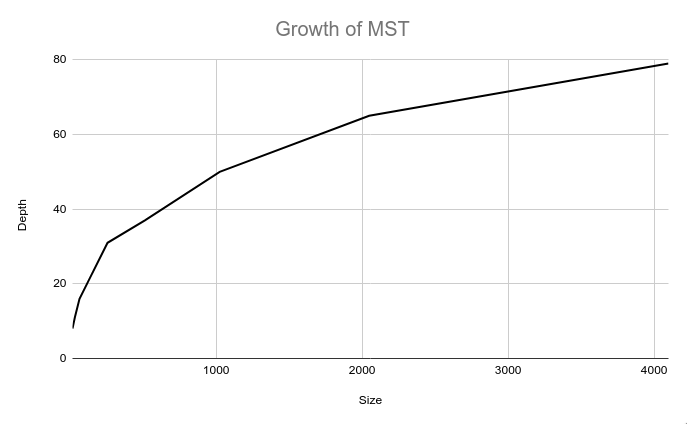
\includegraphics[scale=0.5]{plot}
  \caption{Experiment results.}
  \label{fig:1}
\end{figure}

\section{Results}\label{sec:3}

%%%%%%%%%%%%%%%%%%%%

\bibliographystyle{unsrt}
\bibliography{refs}

\end{document}
